\chapter{CUDA profiling and memory}
\label{ch:c7}
\begin{keybox}
\textbf{Key idea.} ``It's slow'' is not a diagnosis. A profile is: it tells you
\emph{where} a time step's time and memory actually go, so you optimize the
thing that matters instead of the thing you guessed. This chapter profiles one
complete Cahn--Hilliard step with tools that work on any box, teaches the
Nsight Systems commands for the device-level detail, and --- crucially --- shows
that on the tutorial's direct-solver path the GPU is barely the bottleneck at
all.
\end{keybox}

\begin{keybox}
\textbf{Learning objectives.} By the end you can: time one complete step with
CUDA \emph{synchronization} and explain why an unsynchronized timer lies;
measure kernel-launch overhead, device memory bandwidth, and host$\leftrightarrow$device
copy bandwidth, and place a kernel on the memory-bound side of a roofline;
read a sparse-LU factor-vs-solve split and argue for factor reuse; account for
a step's device memory analytically when the mempool hides it; and drive
\texttt{nsys profile}/\texttt{nsys stats} with NVTX ranges to capture one
step's timeline.\\[2pt]
\textbf{Prerequisites.} The Newton step and its assembly/solve stages
(Chapter~\ref{ch:c0}); the solver landscape and cost accounting
(Chapters~\ref{ch:c4},~\ref{ch:c5}); basic GPU execution model (kernels,
launches, host/device memory).\\[2pt]
\textbf{Expected cost.} One CUDA GPU, 2-D, well under 1\,GB of problem memory;
solver \texttt{splu}. \texttt{run.py} completes in $\approx$30--40\,s on an
RTX~6000 Ada, including one \texttt{nsys} capture.
\end{keybox}

This chapter profiles the production step
(\file{src/diffsim/physics/cahn\_hilliard.py}) at level~6 ($\CsevenDofs$ dofs,
$\CsevenNnz$ nonzeros). Every number here is measured with a CUDA-synchronized
timer or a driver memory query, so it reproduces with or without Nsight.

\section{Time one step --- and synchronize, or the timer lies}

CUDA kernels are launched \emph{asynchronously}: the host queues the work and
returns immediately, long before the GPU finishes. A timer wrapped around a
launch with no synchronization therefore measures the \emph{launch}, not the
\emph{work} --- it can report a kernel as ``instant'' while the GPU is still
busy. The fix is a \texttt{synchronize()} before you start and stop the clock;
the course's \texttt{diagnostics.profiling} timers do exactly this. Our
kernel-launch micro-benchmark shows the host-side cost of a single launch is
$\approx\CsevenLaunchUs$\,$\mu$s --- small, but a step that launches thousands of
tiny kernels pays it thousands of times.

Timed properly, one complete level-6 step takes about $\CsevenStepMs$\,ms and
runs $\CsevenNewtonIters$ Newton iterations. Where does that time go? Not where
a GPU course would have you guess.

\section{Data movement rules: bandwidth vs arithmetic intensity}

Two numbers bound everything a kernel can do: how fast it can compute, and how
fast it can move data. Their ratio for the \emph{kernel} is its
\textbf{arithmetic intensity} (flops per byte moved); the ratio for the
\emph{hardware} is where the roofline bends. A streaming triad
$c=a+2b$ touches three arrays and does two flops --- arithmetic intensity
$\CsevenDeviceAI$ flop/byte, deep in the \emph{memory-bound} regime --- and on
this card it sustains $\CsevenDeviceGbs$\,GB/s, near the hardware peak. A finite
element assembly is the same kind of animal: a little arithmetic per node, a lot
of gather/scatter, memory-bound.

The lesson sharpens when the data has to cross the PCIe bus. A
host$\leftrightarrow$device copy sustains only $\CsevenPcieGbs$\,GB/s ---
$\CsevenBwRatio\times$ slower than on-device memory
(Fig.~\ref{fig:c7bandwidth}). Every Newton iteration of the \texttt{splu} path
copies the assembled element Jacobians back to the host to build the sparse
matrix: $\CsevenDtwohPerStep$\,MB per step across that slow link. Data movement,
not flops, is what you profile for.

\begin{figure}[h]\centering
  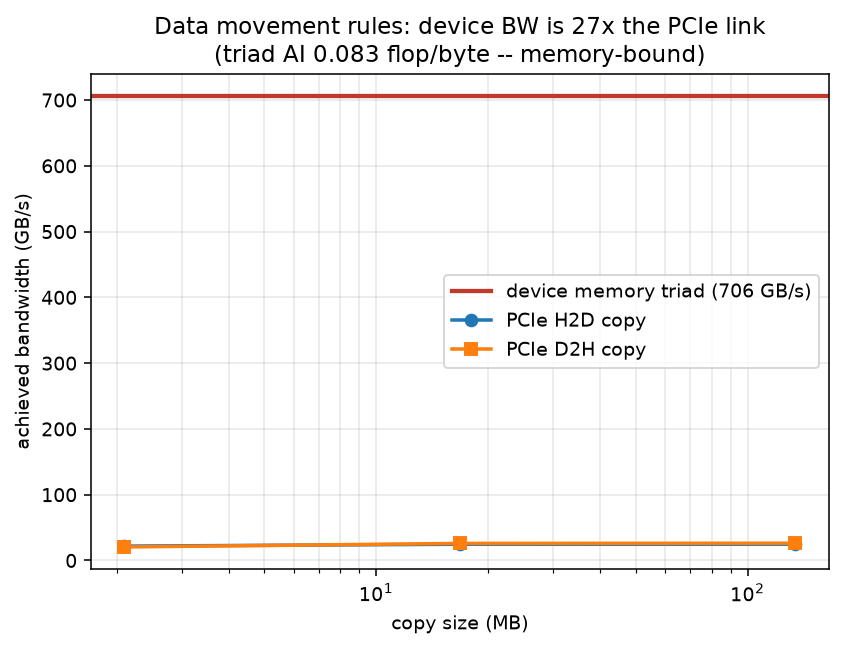
\includegraphics[width=0.72\linewidth]{figures/c7_bandwidth.png}
  \caption{Bandwidth is the currency. The device memory triad (red) sustains
    $\CsevenDeviceGbs$\,GB/s near the card's peak; a host$\leftrightarrow$device
    PCIe copy saturates at $\CsevenPcieGbs$\,GB/s, $\CsevenBwRatio\times$ slower.
    With arithmetic intensity $\CsevenDeviceAI$ flop/byte the triad is
    memory-bound --- moving the data, not doing the math, sets the time.}
  \label{fig:c7bandwidth}
\end{figure}

\section{Factor vs solve: the case for reuse}

On the tutorial's direct-solver path the real cost is neither on the GPU nor on
the bus --- it is the host sparse-LU \emph{factorization}. Factoring the level-6
saddle system costs $\CsevenFactorMs$\,ms; a triangular \emph{solve} with that
factor costs only $\CsevenSolveMs$\,ms --- a $\CsevenFactorRatio\times$ ratio.
Because the Cahn--Hilliard tangent changes every Newton iteration, the stepper
refactors each time: $\CsevenNewtonIters$ factorizations for one step. That is
the single biggest line in the step's budget (Fig.~\ref{fig:c7breakdown},
left), and it is why the GPU sits nearly idle on this path.

Two honest conclusions follow, both pointing forward. First, when a matrix (or
its symbolic structure) is reused --- a frozen tangent, a modified-Newton
scheme, or a solver that caches its symbolic factorization --- you pay the
factor cost once and amortize it over many cheap solves. Second, a GPU direct
solver (cuDSS) or an iterative device solver moves this dominant cost onto the
hardware the tutorial has been provisioning all along (Chapter~\ref{ch:c4}).
Profiling did not just measure the step; it \emph{redirected} the optimization.

\begin{figure}[h]\centering
  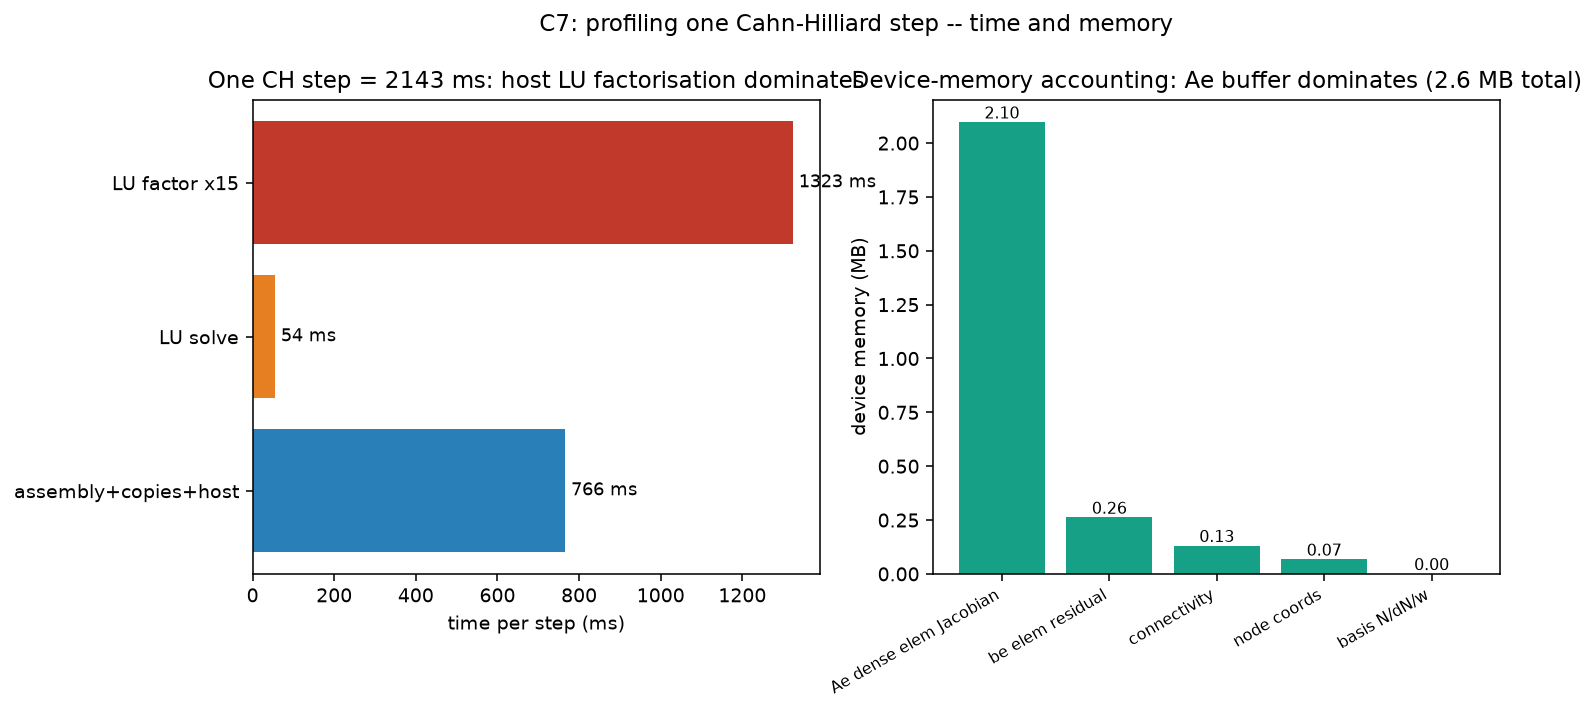
\includegraphics[width=\linewidth]{figures/c7_breakdown.png}
  \caption{Profiling one step. \emph{Left:} the step-time budget --- host LU
    factorization (repeated once per Newton iteration) dominates; the
    triangular solves and the GPU assembly/copies are a sliver. \emph{Right:}
    the device-memory accounting --- the dense per-element Newton Jacobian
    buffer \texttt{Ae} ($\CsevenAeMb$\,MB) dwarfs the mesh and basis arrays.}
  \label{fig:c7breakdown}
\end{figure}

\section{Device memory: measure it, or account for it}

Peak device memory is the number that decides whether a problem fits. It is
also the one a naive query gets wrong: Warp manages device memory through a
\emph{caching mempool}, so an in-process ``used-memory'' delta reads $\approx0$
(the pool recycles freed buffers) and a driver query is quantized to the pool's
reservation granularity. Measured in a \emph{fresh} process, the level-6 step's
driver footprint is $\CsevenDriverMb$\,MB; the honest, reproducible number is an
\textbf{analytical accounting} of the arrays the code allocates
($\CsevenAnalyticalMb$\,MB total), dominated by the dense element-Jacobian
buffer \texttt{Ae} at $\CsevenAeMb$\,MB (Chapter~\ref{ch:c5}'s memory discipline,
on the device side). The two agree because \texttt{Ae} \emph{is} the step's
dominant transient allocation. When the mempool hides the high-water mark, you
account for it.

\section{Nsight Systems: capture one step}

For the device-level timeline --- which kernels ran, how long, what memory
copies moved --- the tool is Nsight Systems. The discipline is to profile
\textbf{one complete step}, not a whole run: JIT-warm the kernels with a
throwaway step, wrap the step you care about in an NVTX range, and profile that.
\file{nsys\_workload.py} does exactly this, marking \texttt{warmup} and
\texttt{ch\_step} ranges. Capture and summarize with:
\begin{lstlisting}
nsys profile --trace=cuda,nvtx --sample=none --force-overwrite=true \
    -o outputs/c7/step_profile  <repo>/.venv/bin/python nsys_workload.py
nsys stats --report nvtx_sum --report cuda_gpu_kern_sum \
    outputs/c7/step_profile.nsys-rep
\end{lstlisting}
On the course box this capture succeeds (\texttt{nsys\_captured =
\CsevenNsysCaptured}) and the NVTX summary reports the two ranges directly ---
the profiled \texttt{ch\_step} at $\approx\CsevenNvtxStep$\,ms, the compile-heavy
\texttt{warmup} at $\approx\CsevenNvtxWarmup$\,ms.

\begin{keybox}
\textbf{On kernel-level rows.} The per-kernel and per-memcpy tables
(\texttt{cuda\_gpu\_kern\_sum}, \texttt{cuda\_gpu\_mem\_time\_sum}) require a
CUPTI that matches your CUDA \emph{driver}. On a box whose driver is newer than
the installed Nsight, \texttt{nsys stats} reports ``does not contain CUDA kernel
data'' while still giving the NVTX timeline (as here). The commands are
unchanged --- on a matched toolchain the same two reports print the per-kernel
breakdown. Run them on your box; the NVTX timing and the synchronized timers in
this chapter carry the quantitative story either way.
\end{keybox}

\begin{runbox}
\textbf{Run it.}
\begin{lstlisting}
cd computational/07_cuda_profiling
python run.py --config configs/c7.yaml --device cuda:0 \
    --solver splu --output outputs/c7 --overwrite --mode reference
python gen_figures.py --run-dir outputs/c7
\end{lstlisting}
It times one synchronized step, measures launch overhead / bandwidth / the
factor-vs-solve split / the device-memory footprint, and runs one
\texttt{nsys} capture; it prints \texttt{PASS/FAIL} gates for the invariants
(bandwidth $\gg$ PCIe, memory-bound triad, factor $\gg$ solve) and checks
\file{baseline.yaml}. Compare with \file{EXPECTED.md}.
\end{runbox}

\begin{keybox}
\textbf{Measured self-check} (hardware-dependent; the \emph{ratios} are the
load-bearing quantities).
\begin{center}\small
\begin{tabular}{lcl}
\toprule
quantity & measured & invariant \\
\midrule
one step & $\CsevenStepMs$\,ms, $\CsevenNewtonIters$ its & --- \\
launch overhead & $\CsevenLaunchUs$\,$\mu$s & per launch \\
device / PCIe BW & $\CsevenDeviceGbs$ / $\CsevenPcieGbs$\,GB/s & $\CsevenBwRatio\times$ gap \\
triad intensity & $\CsevenDeviceAI$ flop/byte & memory-bound \\
factor / solve & $\CsevenFactorMs$ / $\CsevenSolveMs$\,ms & $\CsevenFactorRatio\times$ \\
device memory & $\CsevenAnalyticalMb$\,MB (\texttt{Ae} $\CsevenAeMb$) & accounted \\
\bottomrule
\end{tabular}
\end{center}
\end{keybox}

\section{Explore on your own}

\question{Re-time the step \emph{without} the CUDA synchronization (drop the
\texttt{sync} in the timer). By how much does the reported time change, and in
which direction? Explain the sign from the async launch model.}

\question{Sweep the mesh level $5\to7$ and plot step time, factor time, and the
analytical device memory against the dof count. Which grows fastest, and does
the factor-vs-solve ratio hold?}

\question{Switch the solver to a device path (Chapter~\ref{ch:c4}) and
re-profile. Does the host factorization line in Fig.~\ref{fig:c7breakdown}
shrink? What becomes the new dominant cost, and is it now on the GPU?}

\question{The triad reaches $\CsevenDeviceGbs$\,GB/s. Estimate the card's peak
memory bandwidth from its spec and compute the fraction achieved. What would a
\emph{compute}-bound kernel (high arithmetic intensity) look like on the same
plot?}

\question{On your own box, run the two \texttt{nsys stats} reports. If the
per-kernel table prints, which kernel dominates \texttt{ch\_step}, and is it the
assembly or something else? If it reports ``no CUDA kernel data,'' what does
that tell you about your Nsight/driver versions?}
